\chapter{INTRODUÇÃO}
\label{chapter:introducao}

A robótica e o estudo de mecanismos articulados são áreas fundamentais da engenharia moderna, com aplicações que variam desde a automação industrial até a exploração aeroespacial. O projeto e o controle precisos desses sistemas exigem uma compreensão profunda do seu comportamento físico, o que é alcançado através da modelagem dinâmica. A disciplina de Dinâmica fornece as ferramentas matemáticas necessárias para prever as trajetórias, velocidades, acelerações e as forças envolvidas no movimento de corpos rígidos no espaço.

Neste contexto, a construção de protótipos físicos de baixo custo surge como uma excelente metodologia ativa de aprendizagem, permitindo a correlação direta entre a teoria matemática e a prática \cite{meriam2012,hibbeler2016}. O presente relatório documenta a modelagem dinâmica de um mecanismo robótico simples, construído com palitos de picolé e de churrasco, e acionado por um motor DC com caixa de redução. Apesar da simplicidade dos materiais, o sistema preserva toda a complexidade cinemática e cinética de um manipulador robótico real, exigindo o equacionamento rigoroso de seus elos (corpos rígidos) através das formulações vetoriais de Newton-Euler.

O mecanismo estudado é inspirado em robôs educacionais que se deslocam ao longo de uma corda. Um motor com caixa de redução gira duas manivelas defasadas de 180$^\circ$; cada manivela move um braço, que funciona como alavanca em torno do eixo do quadril e termina em um gancho apoiado na corda, enquanto duas pernas penduradas atuam como contrapesos. Com o motor girando no sentido anti-horário, os braços se alternam, um indo para trás enquanto o outro vai para a frente, e o robô avança sobre a corda. Neste trabalho escolhem-se o centro de massa do robô e a ponta das mãos (a extremidade superior dos braços) como pontos de interesse, e o objetivo é prever o deslocamento desses pontos.

\section{Objetivos}

\subsection{Objetivo Geral}
O presente trabalho tem como objetivo geral aplicar os conceitos fundamentais da dinâmica dos corpos rígidos \cite{beer2013} para modelar, equacionar e analisar o movimento de um mecanismo robótico articulado, construído a partir de materiais de baixo custo e acionado por um motor DC com redução.

\subsection{Objetivos Específicos}
Para alcançar o objetivo geral proposto e cumprir as etapas de desenvolvimento, definem-se os seguintes objetivos específicos:
\begin{itemize}
    \item Projetar e construir o protótipo físico do mecanismo robótico, partindo da seleção e aquisição de insumos de baixo custo;
    \item Determinar a massa, o centro de massa e o tensor de inércia de cada peça e do conjunto montado, a partir das medidas do protótipo;
    \item Realizar testes práticos e filmagens do protótipo em operação, visando a extração do comportamento real do sistema para posterior comparação teórica;
    \item Desenvolver, testar e validar um código computacional dedicado à resolução analítica das equações vetoriais de cinemática e cinética (Leis de Newton-Euler);
    \item Simular o movimento do robô sobre a corda, com o motor a 30 rpm no sentido anti-horário, e apresentar o deslocamento do centro de massa e da ponta das mãos;
    \item Documentar estruturalmente todo o desenvolvimento do projeto, englobando a fundamentação teórica, a metodologia construtiva e as revisões de código, culminando na elaboração e entrega deste relatório técnico.
\end{itemize}

\section{Cronograma de Atividades}

Para garantir o cumprimento de todos os objetivos específicos dentro do prazo estabelecido pela disciplina, o desenvolvimento do projeto foi estruturado através de um planejamento estratégico das tarefas. 

A \ref{fig:gantt} apresenta o diagrama de Gantt do projeto, ilustrando a linha do tempo desde a aquisição dos insumos e início da escrita do código, passando pela construção e filmagem do robô, até as etapas finais de revisão geral e entrega do relatório.

\begin{figure}[H]
\begin{center}
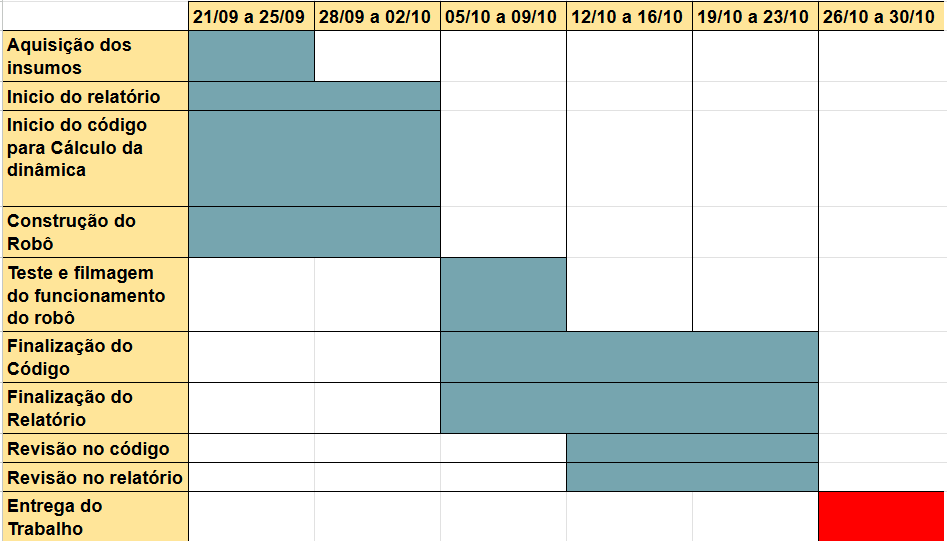
\includegraphics[width=13cm]{gantt.png}
\caption{\label{fig:gantt}- Diagrama de Gantt com o cronograma de atividades do projeto.}
\end{center}
\end{figure}

\section{Organização do Trabalho}

O Capítulo \ref{chapter:revisao} apresenta a fundamentação teórica: a cinemática e a cinética do corpo rígido, o tensor de inércia e o equacionamento de um sistema de corpos. O Capítulo \ref{chapter:metodologia} descreve a construção do protótipo e o levantamento das massas e das dimensões. O Capítulo \ref{chapter:inercia} reúne o cálculo dos tensores de inércia de cada peça e do robô montado. O Capítulo \ref{chapter:modelo} desenvolve o modelo cinemático e dinâmico, e o Capítulo \ref{chapter:resultados} apresenta e discute os resultados da simulação. Por fim, são apresentadas as conclusões e, no Apêndice \ref{ap:codigo}, a estrutura do código utilizado.
